\section{Deep Recurrent Attentive Writer }

From the previous section on the convolutional autoencoder it is clear that we can encode class information latent spaces. The remaining question is then whether we can cluster these representations, or if we can improve the separation in other ways. One way of discovering the latter is with a recurrent model like DRAW (deep recurrent attentive writer) as discussed in section \ref{sec:draw}. We discuss the former in the next chapter, which focuses entirely on the clustering of AT-TPC events.

In the same manner as for the convolutional autoencoder this section begins by considering the semi-supervised classification results using a flattened representation of the sequence of latent samples. To build on those results we also investigate the performance as a function of latent samples and whether these are densely packed in class separated clusters.

As the algorithm is sequential we elected to concatenate the latent samples to a single vector for classification purposes.

The hyperparameters of the algorithm were determined with a random search architecture, in a manner equivalent to how we determined the values for the convolutional autoencoder. To keep the search-space feasible we froze some of the hyperparameters pertaining to the architecture in the read-write function pair. For the convolutional architecture we used four layers with stride $s=2$ and kernel sizes $k= [5,\, 5,\, 3,\, 3]$. For the attention parameters we specified a glimpse size of $\delta=0.8$ and searched over the number of Gaussian filters $N$. The simulated and full datasets achieved optimal performance with a convolutional read/write configuration, while the filtered data showed the strongest performance with attention parameters. For the filtered data the search yielded filter values $N_{read} = 15$ and $N_{write}=20$. And for the full and simulated data the optimal value for the convolutional filters was $f=8$ for all layers. The remainder of the hyperparameters are presented in table \ref{tab:best_draw_hyperparams}.


\begin{table}
\centering
\caption{Hyperparameters that yielded the optimal performance on the semi-supervised task for the DRAW algorithm}\label{tab:best_draw_hyperparams}
\begin{tabular}{llll}
\toprule
Hyperparameter & Simulated & Filtered & Full \\
\midrule
\multicolumn{4}{l}{Recurrent parameters: } \\
\midrule
$Dim(\text{encoder})$ & $128$ & $512$ & $256$ \\
$Dim(\text{decoder})$ & $64$ & $512$ & $256$ \\
\midrule
\multicolumn{4}{l}{Network parameters: } \\
\midrule
Latent type & MMD & None & MMD  \\
Latent dimension & $100$ & $100$ & $10$ \\
$\beta$ & $10$ & None $100$\\
Batchnorm & False & False & True \\
\midrule
\multicolumn{3}{l}{Optimizer parameters: } \\
\midrule
$\eta$ & $\num{1e-3}$ & $\num{1e-5}$ & $\num{1e-2}$ \\
$\beta_1$ & $0.92$ & $0.94$ & $0.81$ \\
$\beta_2$ & $0.99$ & $0.99$ & $0.99$ \\
\bottomrule
\end{tabular}
\end{table}

We begin by considering the $f1$ scores of the logistic regression classifier on the latent samples. These scores are included in table \ref{tab:draw_clf}, where we note that there seems to be no large deviation from the non-sequential autoencoder. 

\begin{table}
\centering
\caption{Logistic regression classifier performance on the latent space of the DRAW algorithm.}\label{tab:draw_clf}
\begin{tabular}{lllll}
\toprule
{} &                                              Proton &                                              Carbon &                                               Other &                                                 All \\
\midrule
Simulated &  $\underset{\num{+- 1.297e-02 }  }{\num{ 0.548 } }$ &  $\underset{\num{+- 1.759e-02 }  }{\num{ 0.615 } }$ &  N/A &  $\underset{\num{+- 1.528e-02 }  }{\num{ 0.582 } }$ \\
Filtered  &  $\underset{\num{+- 2.244e-02 }  }{\num{ 0.378 } }$ &  $\underset{\num{+- 5.943e-02 }  }{\num{ 0.364 } }$ &  $\underset{\num{+- 4.885e-02 }  }{\num{ 0.617 } }$ &  $\underset{\num{+- 4.358e-02 }  }{\num{ 0.453 } }$ \\
Full      &  $\underset{\num{+- 9.023e-04 }  }{\num{ 0.434 } }$ &  $\underset{\num{+- 0.000e+00 }  }{\num{ 0 } }$ &  $\underset{\num{+- 0.000e+00 }  }{\num{ 0 } }$ &  $\underset{\num{+- 3.008e-04 }  }{\num{ 0.145 } }$ \\
\bottomrule
\end{tabular}

\end{table}

Additionally, we wish to characterize the latent space by how many latent samples it takes to achieve this optimal performance. We present these performance records in figure \ref{fig:draw_nsamples}. 

\begin{figure}
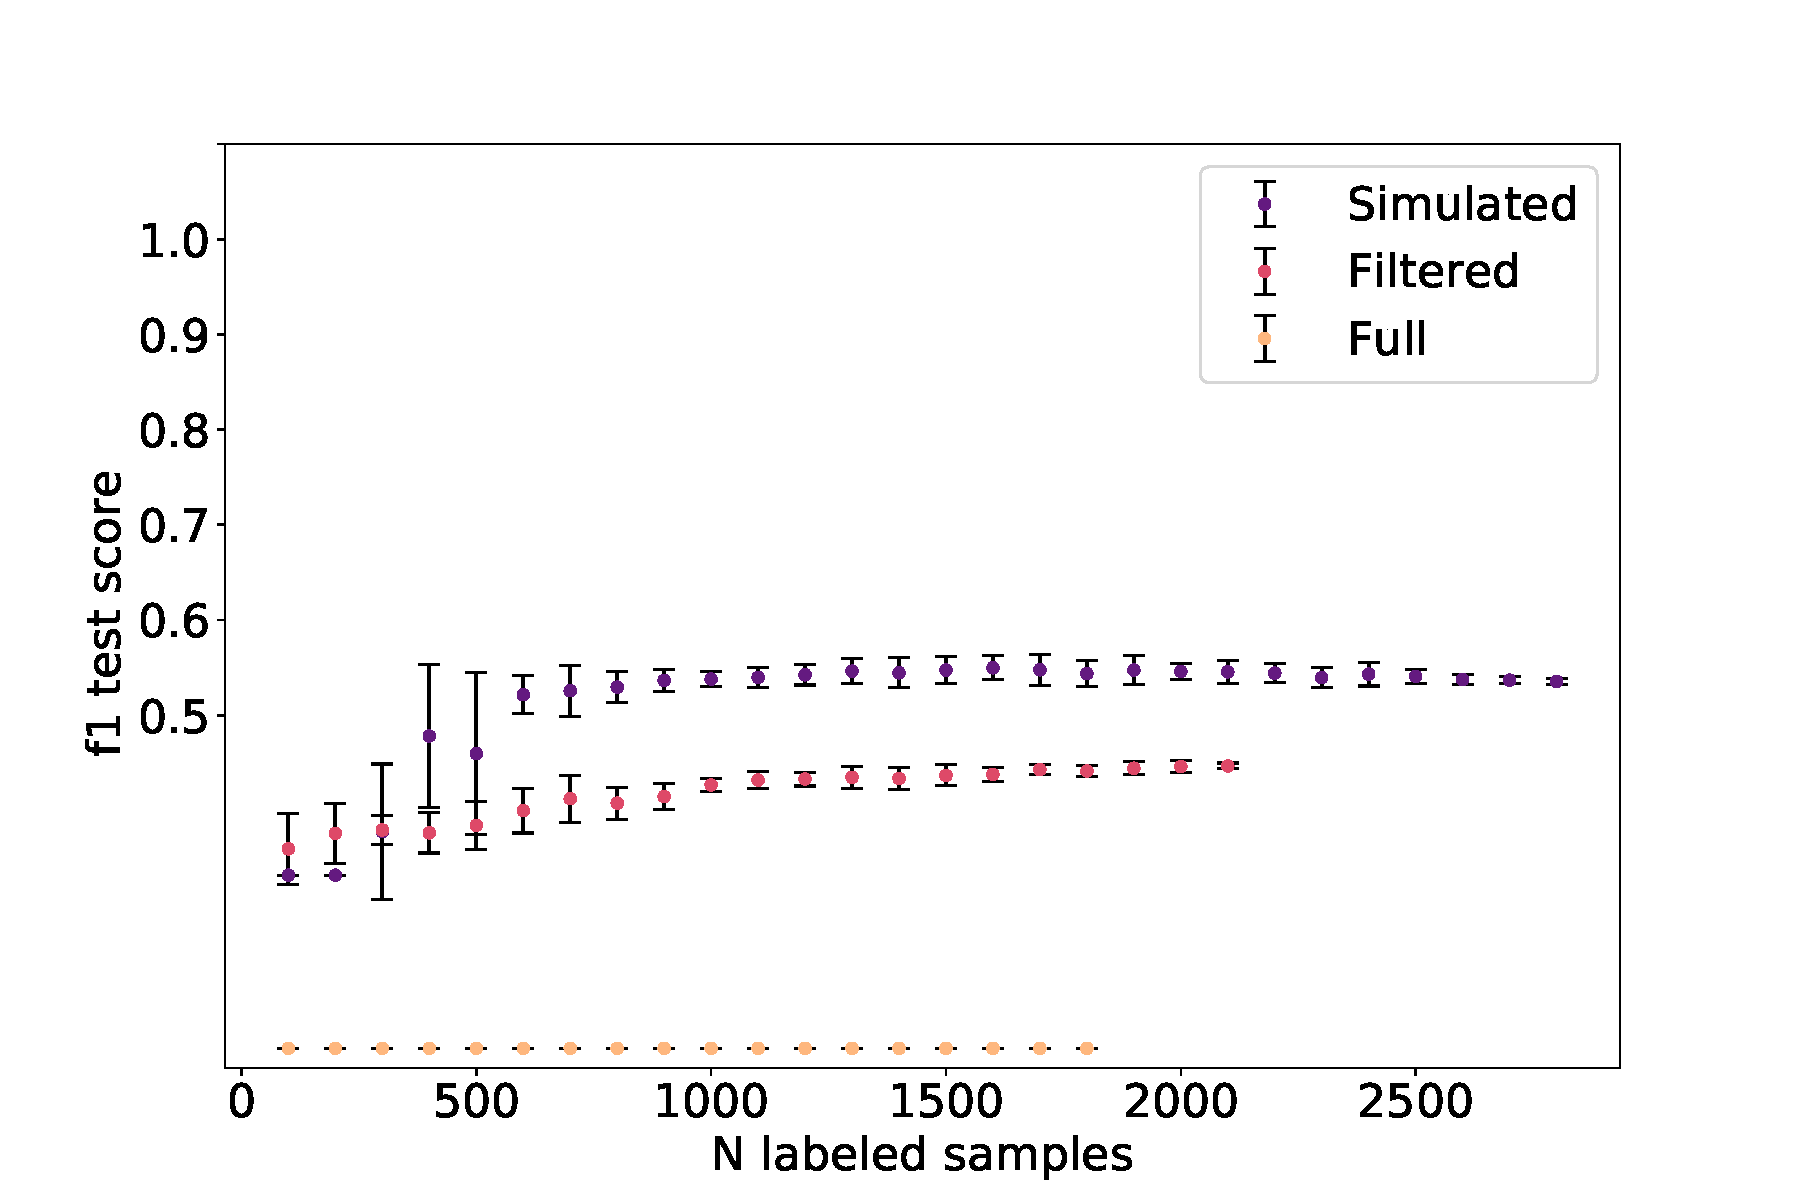
\includegraphics[width=\textwidth]{plots/ac_draw_n_samples.pdf}
\caption[Semi supervised classification with DRAW]{Performance of the logistic regression algorithm on the three datasets as a function of number of latent samples. The latent samples are produced with the DRAW algorithm using the hyperparameters presented in table \ref{tab:best_draw_hyperparams}}\label{fig:draw_nsamples}
\end{figure}


Lastly we wish to describe the latent space in some detail. Like with the VGG16 latent space and the non-sequential convolutional autoencoder we project the latent space to a low-dimensional space. The projection is made with the t-SNE algorithm, and the results are presented in figure 


\begin{figure}
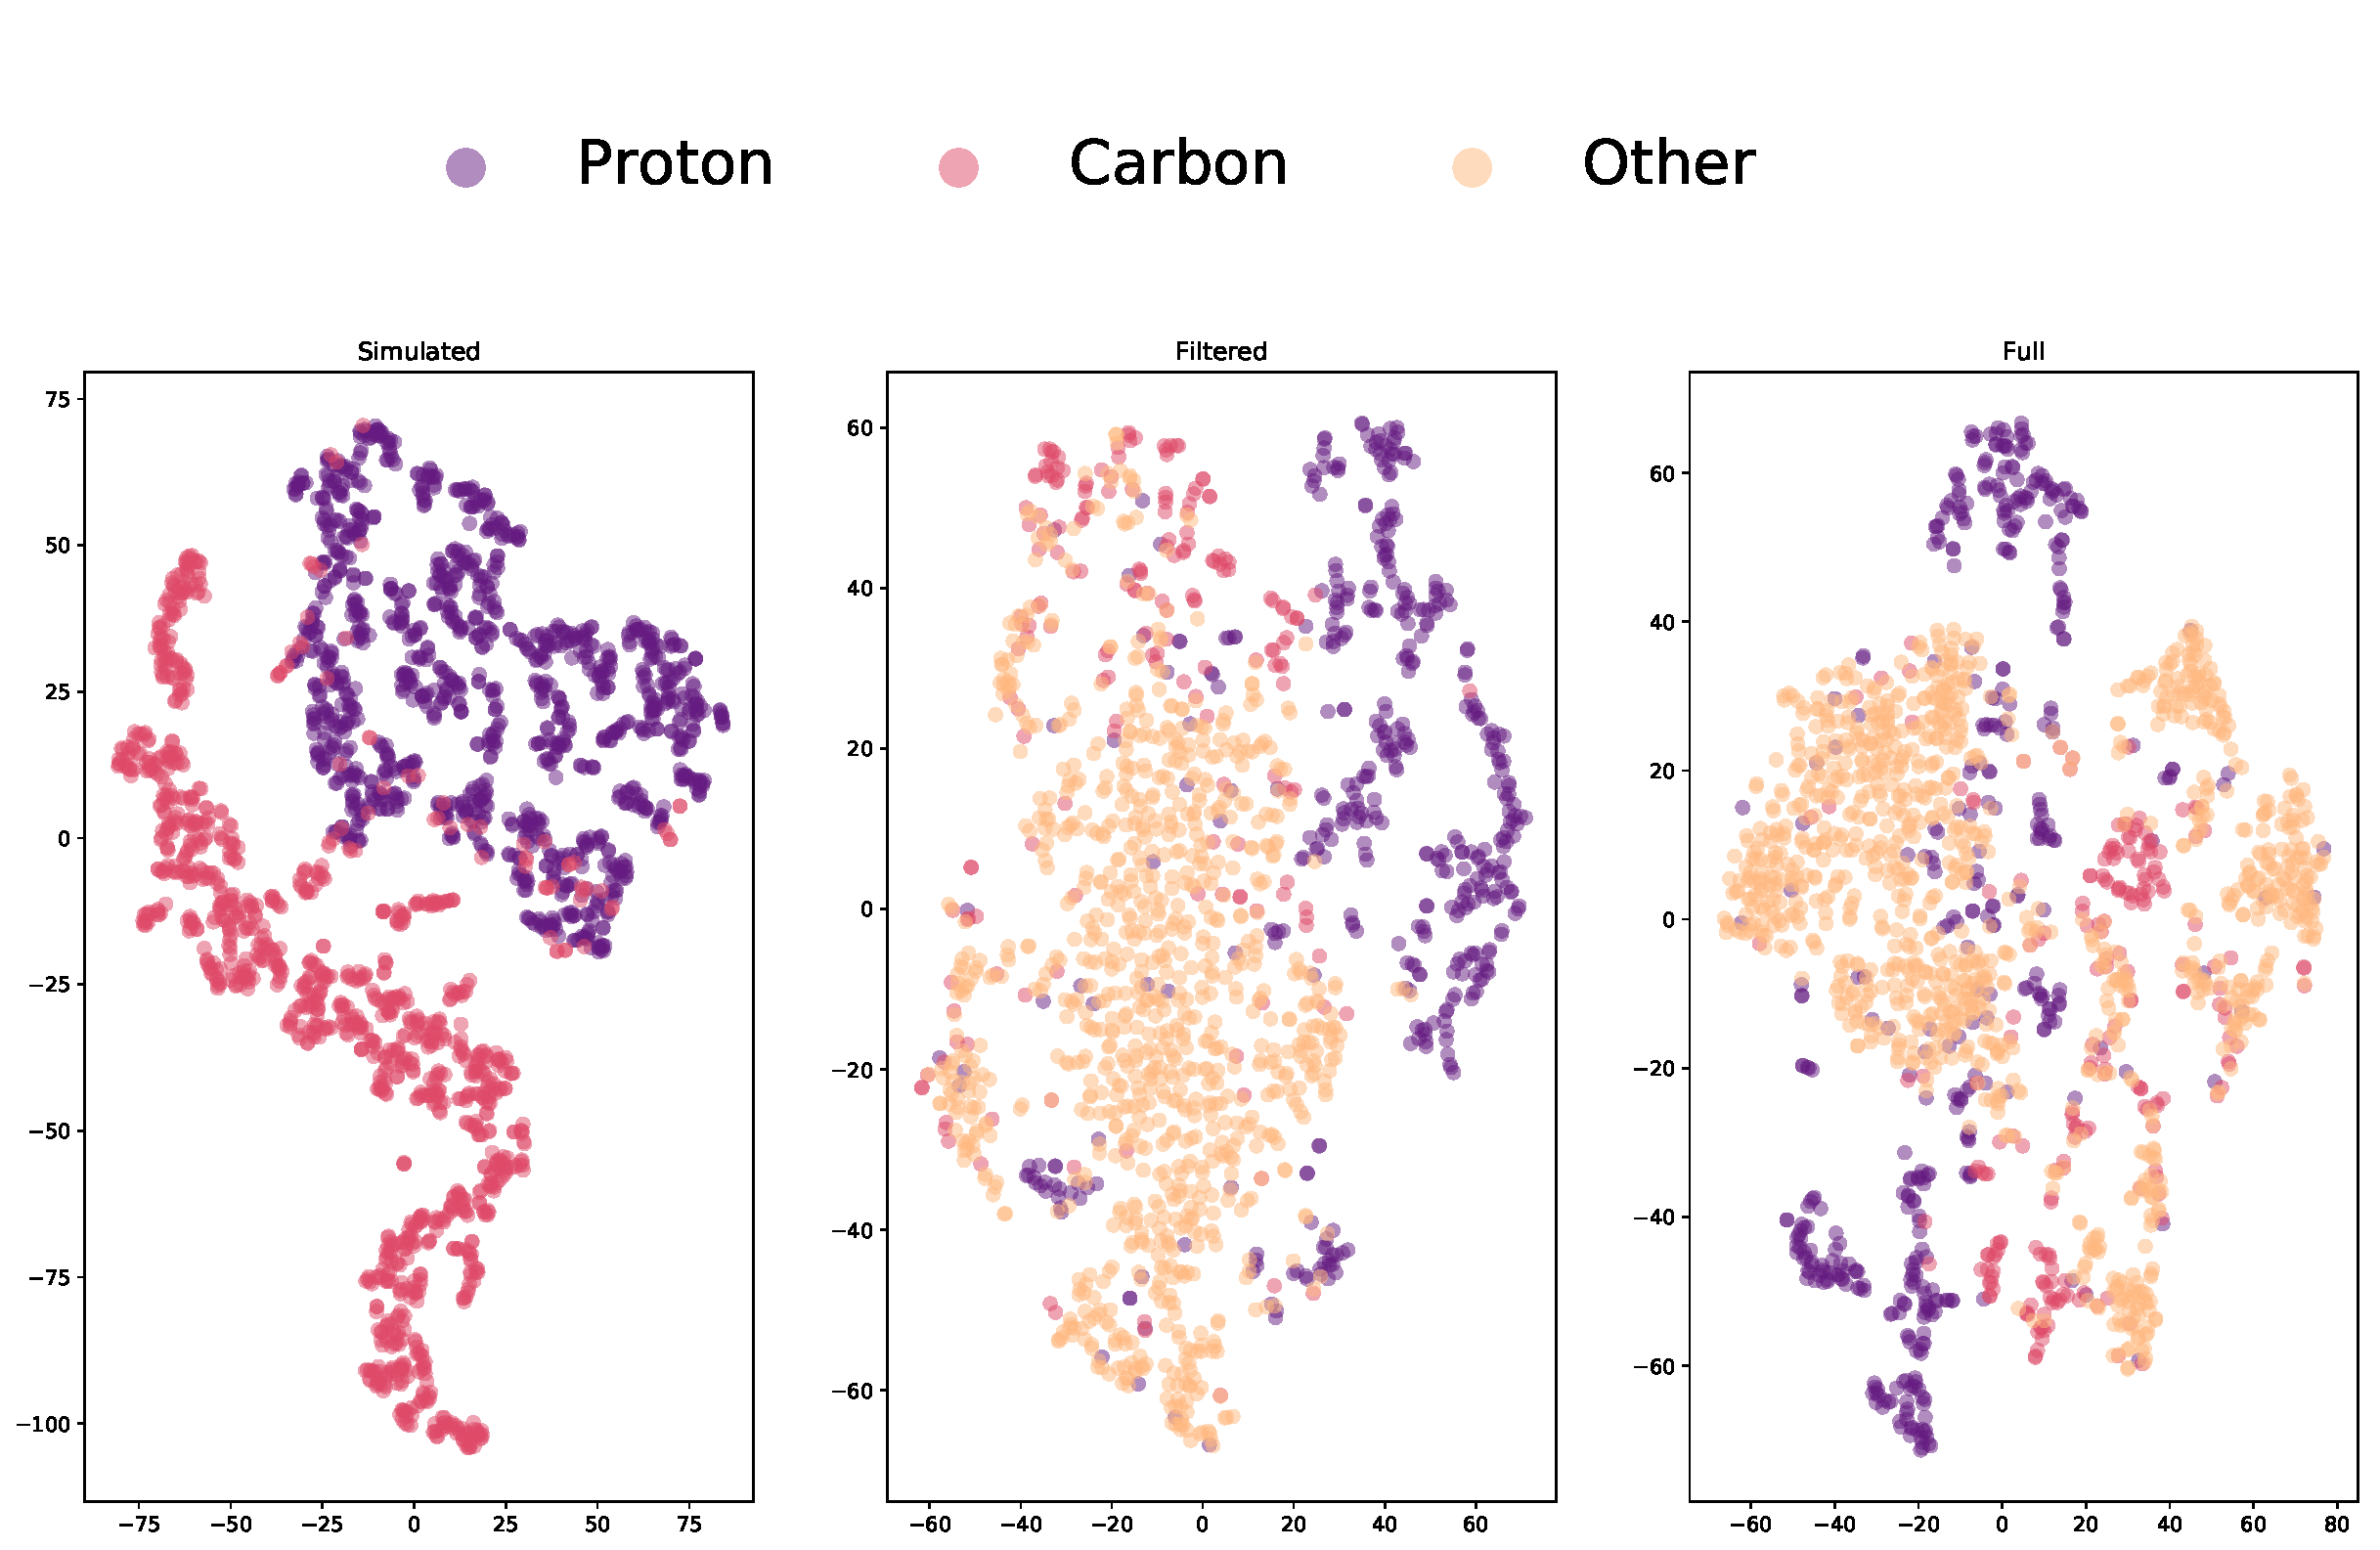
\includegraphics[width=\textwidth]{plots/ac_tsne_draw.pdf}
\caption[t-SNE projection of the DRAW latent space]{t-SNE projection of the DRAW latent space.  The latent samples are produced with the DRAW algorithm using the hyperparameters presented in table \ref{tab:best_draw_hyperparams}}
\end{figure}
